%%%%%%%%%%%%%%%%%%%%%%%%%%%%%%%%%%%%%%%%%%%%%%%%%%%%%%%%%%%%%%%%%%%%%
%%                                                                 %%
%%                                                                 %%
%%               Sujets Maths-en-Jeans                             %%
%%                   Alexandre Pasco                               %%
%%                                                                 %%
%%                                                                 %%
%%                                                                 %%
%%%%%%%%%%%%%%%%%%%%%%%%%%%%%%%%%%%%%%%%%%%%%%%%%%%%%%%%%%%%%%%%%%%%%


\documentclass[a4paper,10pt,oneside]{article}
%
% This is a basic set of packages.  Feel free to use as many packages
% as you want, only the generated PDF will be submitted in the end.
%
\usepackage[utf8]{inputenc}
\usepackage[margin=25.4mm]{geometry}
\usepackage{titlesec}
\usepackage{amsmath,amssymb}
\usepackage{xcolor,graphicx}
\usepackage{amsfonts}
\usepackage{amsthm}
\usepackage{amsopn}
\usepackage[caption=false]{subfig}
\usepackage{bbm}
\usepackage{lipsum}
\usepackage{hyperref}
%\hypersetup{hidelinks}
\usepackage[capitalize,nameinlink]{cleveref}
\usepackage{anyfontsize}
\usepackage[labelfont=bf]{caption}


\title{Sujets Maths en Jeans 2023-2024}

\author{
  Alexandre Pasco${}^{1}$}

\date{\medskip%
  \small %
  ${}^1$  Centrale Nantes, Nantes Université, Laboratoire de Mathématiques Jean Leray\\
  \texttt{Alexandre.Pasco@ec-nantes.fr}
  }

%%%% My commands
\newcommand{\sectionbreak}{\clearpage}

%%%% Theorems
\newtheorem{theorem}{Theorem}
\newtheorem{proposition}[theorem]{Proposition}% 
\newtheorem{corollary}[theorem]{Corollary}%
\newtheorem{example}{Example}%
\newtheorem{remark}{Remark}%
\newtheorem{definition}{Definition}%

%%%% Document
\begin{document}

\maketitle


\section{Ta fête}
Vous invitez aléatoirement des personnes à votre anniversaire. 
Combien de personnes faut-il inviter pour être sûr d'avoir au moins un groupe de $3$ personnes qui se connaissent (ou ne se connaissent pas) mutuellement ? 

\vspace{3cm}
\begin{figure}[!ht]
  \centering
  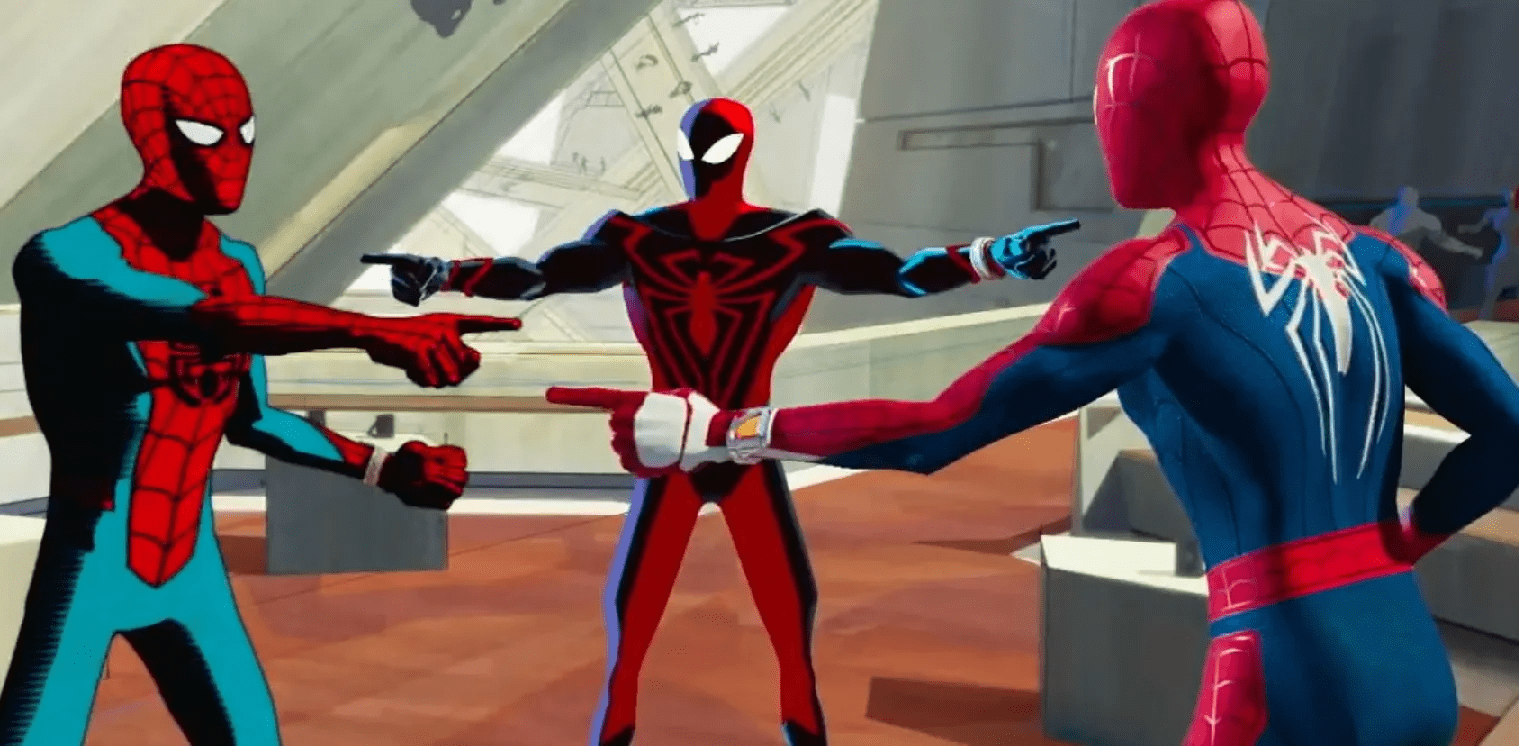
\includegraphics[width=0.9\textwidth]{figures/fete.png}
  \caption*{Image tirée du film \textit{Spider-Man : Across the Spider-Verse}.}
\end{figure}


\section{Traders en herbe}

Vous êtes $n$ joueurs et chacun de vous a un nombre fétiche entre $1$ et $n$. 
Deux joueurs ne peuvent pas avoir le même nombre fétiche.
Vous tirez aléatoirement $1$ carte dans un paquet contenant $n$ cartes numérotées de $1$ à $n$. Votre but est que tous les joueurs obtiennent leur nombre fétiche.
Pour ce faire vous pouvez faire des échanges entre vous.

\paragraph*{1)} 
Pouvez-vous réussir en n'effectuant que des échanges deux à deux ? 
Si oui, proposez une stratégie qui marcherait pour tout nombre de joueurs.

\paragraph*{2)} 
Pouvez-vous réussir en n'effectuant que des échanges par groupes de trois ?
Si oui, proposez une stratégie qui marcherait pour tout nombre de joueurs.

\vspace{3cm}
\begin{figure}[!ht]
  \centering
  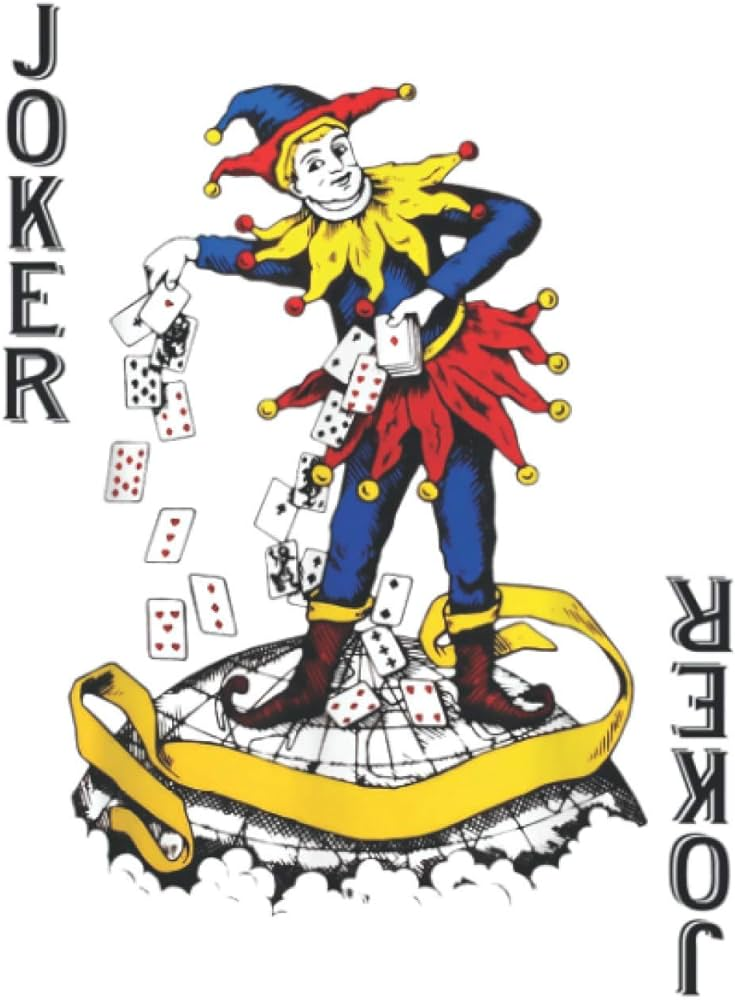
\includegraphics[height=0.5\textheight]{figures/traders.jpg}
  \caption*{Image tirée du site \textit{amazon.fr}}
\end{figure}



\section{Une nouvelle librairie en ville}


Vous êtes le maire d'une ville de 3 habitants, Adrien, Benoît et Clément,  vivant le long d'une route.
Vous voulez y construire une nouvelle librairie pour faire plaisir aux habitants.
Chaque habitant sera d'autant plus content que la librairie sera proche de sa maison. 
Vous demandez à chaque habitant de mettre un drapeau sur l'emplacement qu'il préférerait.
La libraire sera construite à l'emplacement moyen des drapeaux.

\paragraph*{1)} 
Si Clément connaît les préférences des autres, a-t'il intérêt à mentir sur la sienne ?

\paragraph*{2)} 
Si clément ne connaît pas les préférences des autres, mais qu'il connaît le résultat d'un sondage effectué auprès de tous les habitants, où tout le monde a été honnête, a-t'il encore intérêt à mentir ?

\paragraph*{3)} 
Proposez une nouvelle méthode pour sélectionner l'emplacement de la librairie qui serait moins vulnérable face à Clément.

\paragraph*{4)} 
Généralisez les questions précédentes pour une ville avec plus d'habitants.

\paragraph*{5)} 
En restant à 3 habitants, généralisez les questions 1 et 2 au cas où les habitants vivent non plus le long d'une route, mais dans une ville plus classique dans le plan. 


\vspace{3cm}
\begin{figure}[!ht]
  \centering
  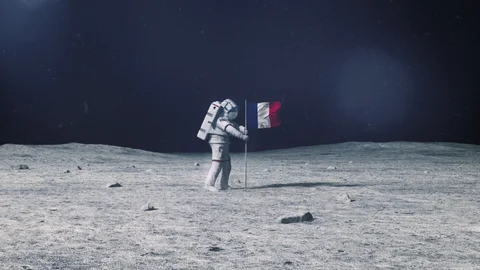
\includegraphics[width=0.9\textwidth]{figures/flag.png}
  \caption*{Image tirée du clip Shutterstock 
  \href{https://www.shutterstock.com/video/clip-1084918624-astronaut-outer-space-on-surface-moon-planting}{1084918624}}
\end{figure}


\section{Le mieux est l'ennemi du bien}

Vous êtes la mairesse d'une ville de 3 habitants.
Un nouveau fast-food va se construire au centre de la ville, et ça ne vous plaît pas.
La construction est inévitable, seul l'emplacement peut être modifié.
Votre but est de l'éloigner autant que possible de l'emplacement d'origine.

Pour ce faire, vous pouvez proposer un nouvel emplacement à vos habitants, qui sera opposé au précédent lors d'un vote à la majorité.
Chaque habitant votera pour l'emplacement le plus proche de chez lui.

Vous pouvez faire voter un nouvel emplacement autant de fois que vous le souhaitez.
Ce dernier sera alors opposé à celui ayant remporté le vote précédent.


\paragraph*{1)} 
Jusqu'où pouvez vous éloigner le fast-food ?

\paragraph*{2)} 
Pouvez-vous généraliser à une ville possédant plus d'habitants ?


\vspace{3cm}
\begin{figure}[!ht]
  \centering
  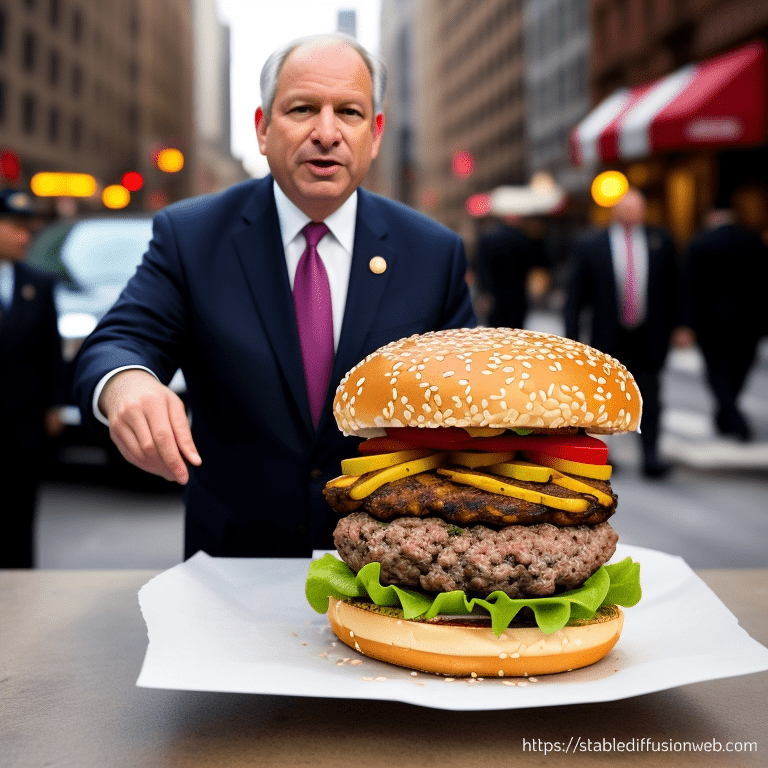
\includegraphics[width=0.75\textwidth]{figures/fast-food.png}
  \caption*{Image générée par le modèle de génération d'image \textit{Stable Diffusion}.}
\end{figure}


\section{Une histoire de boites}

\subsection{Énoncé boites}

Vous êtes une équipe de 4 joueurs devant l'entrée d'une pièce. 
Celle-ci contient 4 boites fermées.
Chacun de vos prénoms est inscrit sur l'une des boites.
Vos prénoms sont également écrits sur 4 papiers (1 prénom par papier), distribués aléatoirement dans les boites (1 papier par boite).

Chacun votre tour, vous entrez dans la pièce et ouvrez 2 boites de votre choix, dans l'ordre de votre choix. 
Vous en lisez le contenu, puis les refermez.
Vous sortez ensuite de la pièce du côté opposé à l'entrée, en laissant tout exactement comme vous l'avez trouvé.
Vous ne pouvez pas interagir avec vos coéquipiers.

L'équipe gagne si tous les joueurs trouvent leu propre prénom dans les boites. Avant de commencer, vous pouvez vous concerter pour choisir une stratégie.

\paragraph*{1)}
Proposez des stratégies et calculez (ou estimez) les chances de victoire correspondantes.
Vous pourrez tester les performances de vos stratégies en faisant des simulations sur ordinateur.

\paragraph*{2)} 
Même question avec un plus grand nombre de joueurs. Pour $n$ joueurs, chacun ouvrira $\frac{n}{2}$ boites.

\vspace{3cm}
\begin{figure}[!ht]
  \centering
  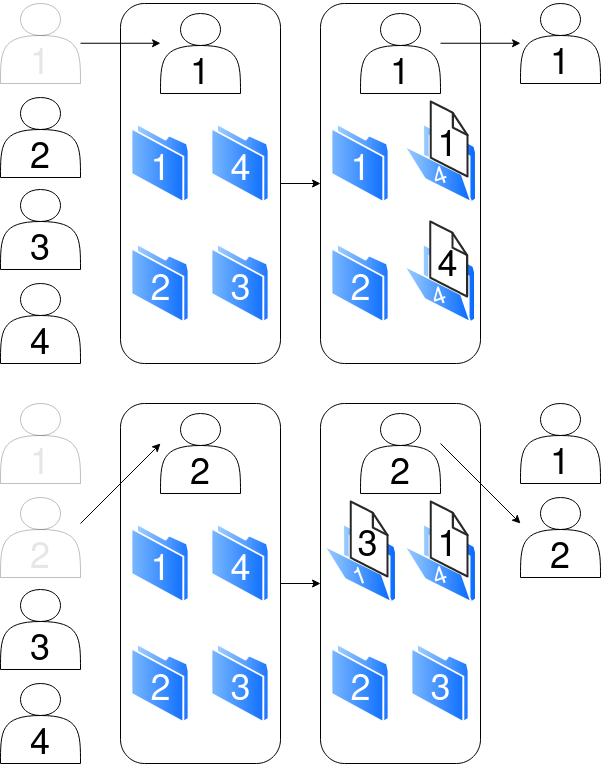
\includegraphics[width=0.9\textwidth]{figures/boites.png}
  \caption*{Image tirée du site \textit{uline.ca}}
\end{figure}

\newpage
\subsection{Énoncé spider-verse}

Vous êtes 4 spider-men et vous venez de sauver le spider-verse en battant le Caïd.
Il est temps pour vous de rentrer dans vos univers respectives.
Vous avez pour cela une machine à voyager entre les dimensions.
Elle se présente sous la forme d'une petite salle, totalement isolée de l'extérieur, qui contient 4 boutons, sur lesquels sont affichés vos univers respectifs.

Le plan est simple: chaque spider-man entre dans la machine, appuie sur le bouton de son univers et traverse le portail dimensionnel qui s'ouvre alors. 
La porte de la machine s'ouvre ensuite et le spider-man suivant peut faire la même chose.

Enfin ça, c'était le plan. 
Il va falloir le changer car, pendant votre combat, le docteur Octopus a mélangé les branchements de la machine.
Résultats, vous ne savez pas à l'avance quel bouton ouvre quel portail.
Vous savez cependant que la machine permet d'ouvrir 2 portails en même temps.
Ainsi, chaque spider-man pourra appuyer sur 2 boutons puis traverse l'un des deux portails ouverts.
Notez que pour des questions de sécurité, vous devez laisser la machine dans l'état exacte dans lequel vous l'avez trouvée.


\paragraph*{1)}
Proposez des stratégies et calculez (ou estimez) les chances que \textbf{tout le monde} rentre dans le bon univers.
Vous pourrez tester les performances de vos stratégies en faisant des simulations sur ordinateur.

\paragraph*{2)} 
Même question avec un plus grand nombre de spider-men. Pour $n$ spider-men, chacun pourra ouvrir $\frac{n}{2}$ portails.

\vspace{3cm}
\begin{figure}[!ht]
  \centering
  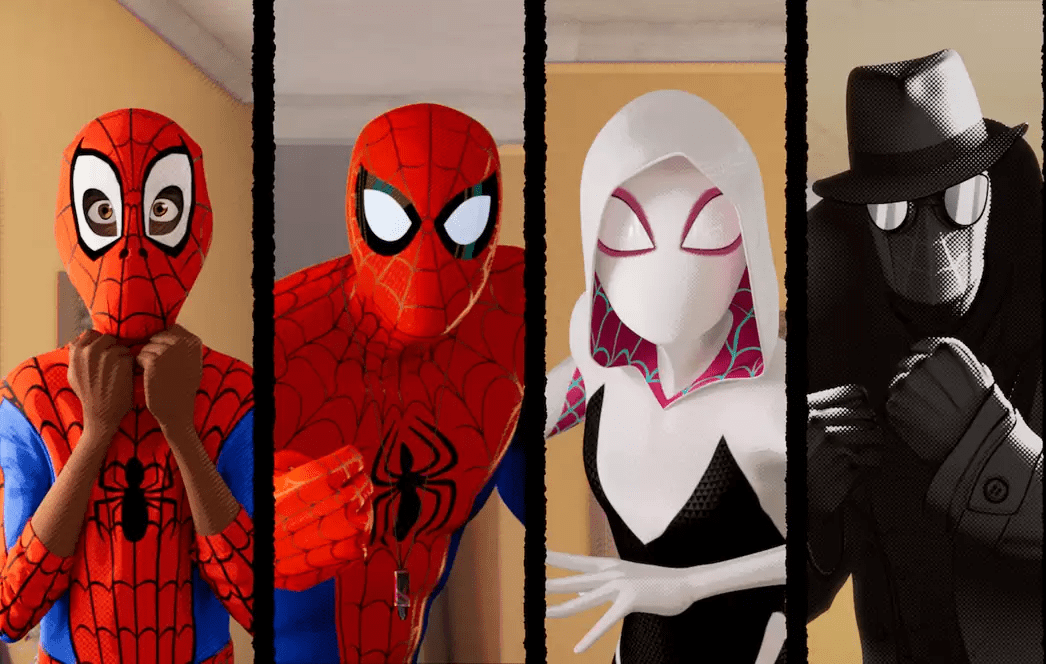
\includegraphics[width=0.9\textwidth]{figures/boites_spider.png}
  \caption*{Miles Morales (1610) | Peter B. Parker (616) | Gwen Stacy (65) | Noir (90214). Image tirée du film \textit{Spider-Man: New Generation}.}
\end{figure}


\section{solutions}

\subsection{Ta fête}

C'est une illustration du 
\href{
  https://fr.wikipedia.org/wiki/Th%C3%A9or%C3%A8me_de_Ramsey#Exemple_:_calcul_de_R(3,3)_=_6
}{théorème des amis et des étrangers}
, qui est lui même un cas particulier du
\href{
  https://fr.wikipedia.org/wiki/Th%C3%A9or%C3%A8me_des_amis_et_des_%C3%A9trangers
}{théorème de Ramsey}.
L'idée est que dès qu'un individu connaît ou ne connaît pas au moins $3$ personnes, alors parmi ces $3+1$ personnes il y a au moins un trio qui se connaissent ou ne se connaissent pas mutuellement.

\subsection{Traders en herbe}

\paragraph*{1)}
Toute permutation peut-être décomposée en transpositions. 
Un stratégie est d'utiliser un pivot qui sera utilisé pour tous les échanges.

\paragraph*{2)} 
Toute permutation ne peut pas être décomposée en cycles de taille 3. 
En effet, un cycle de taille trois est de signature paire (i.e. décomposable en 2 permutations).
Ainsi, une permutation de signature impaire ne pourra pas être décomposée en une composition de tels cycles.


\begin{figure}[!ht]
  \centering
  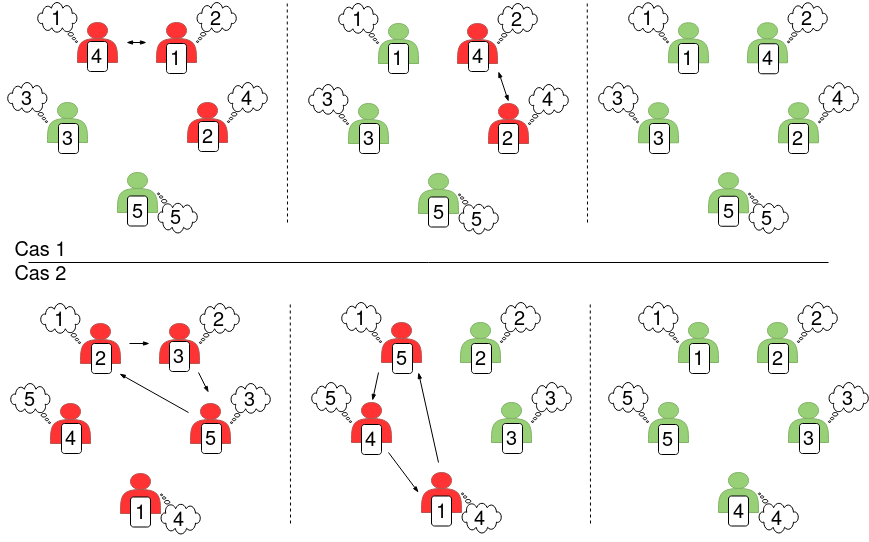
\includegraphics[width=0.9\textwidth]{figures/indice_traders.png}
  \caption{Examples d'échanges à $n=5$ joueurs pour obtenir la distribution désirée. Cas 1, échanges en groupes de 3. Cas 2, échanges en groupes de 3.}
\end{figure}


\subsection{Librairie}

\paragraph*{1,2,4)} 
l'habitant $C$ peut mentir et placer la librairie où il le souhaite. Cela reste vrai avec plus d'habitants.

\paragraph*{3,4)} 
En 1D, une solution moins vulnérable est la médiane des coordonnées. 
Alors, $C$ n'a pas d'intérêt à mentir sur sa vraie préférence. Cela reste vrai avec plus d'habitants.

\paragraph*{5)} 
En 2D pour 3 habitant, une solution moins vulnérable est la médiane géométrique, qui est obtenue en résolvant géométriquement \href{https://fr.wikipedia.org/wiki/Probl%C3%A8me_de_Weber}{le problème de Fermat}. 
C'est la solution qui minimize la somme des distance euclidiennes.
Une autre solution consiste à prendre l'intersection des bissectrices du triangle.

Contrairement au cas 1D, ici Jean a quand même un intérêt à mentir.
Cependant, la zone dans laquelle il peut placer la librairie est bornée.


\begin{figure}[!ht]
\centering
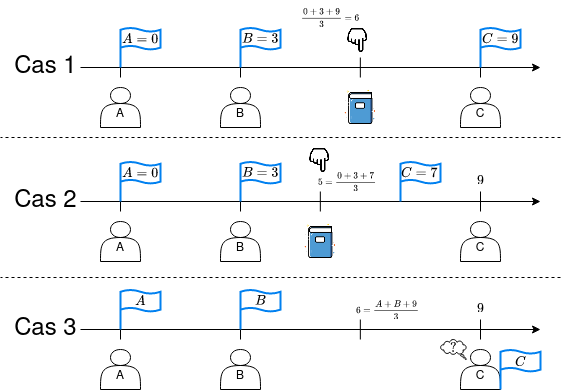
\includegraphics[width=0.50\textwidth]{figures/indice_library.png}
\caption{
  Cas 1, tout le monde est honnête. 
  Cas 2, l'habitant $C$ ment en connaissant les choix de $A$ et $B$. 
  Cas 3, l'habitant $C$ se demande s'il peut gagner à mentir, sachant le résultat du sondage.}
\end{figure}


\subsection{Le mieux est l'ennemi du bien}

Le problème est très bien illustré dans cette \href{https://www.youtube.com/watch?v=goQ4ii-zBMw}{vidéo} qui illustre les résultats de \cite{MCKELVEY1976472}.

\paragraph*{1)} 
Si les habitants ne sont pas alignés, alors peut importe l'emplacement initial, il est possible de faire des propositions d'emplacement successives de sorte qu'il n'y ait pas de limite à l'éloignement de l'emplacement finalement.
Sans aller jusqu'à le prouver rigoureusement, on peut le constater en traçant quelques cercles.

\paragraph*{2)}
La réponse est la même qu'à la question précédente et le processus est semblable.

\begin{figure}[!ht]
  \centering
  \includegraphics*[width=0.95\textwidth]{figures/indice_democracy.png}
  \caption{Deux votes successifs. Une nouvelle proposition est en gris. La proposition votée précédemment est en noir.}
\end{figure}

\subsection{Une histoire de boites}

Si les $n$ joueurs ouvrent aléatoirement les boites, alors leur chance de victoire est $\frac{1}{2^n}$. 
Construire un arbre de probabilités permet d'obtenir ce résultat.
La stratégie optimale consiste à ouvrir la boite sur laquelle est inscrite son numéro, puis ouvrir celle indiquée par le papier, etc. 
Avec cette stratégie, l'équipe de $n$ joueurs à pour probabilité de défaite
\[
  \frac{1}{\frac{n}{2} +1} + \frac{1}{\frac{n}{2} + 2} + \cdots \frac{1}{n} 
  \rightarrow_{n\rightarrow \infty} \ln(2) \simeq 69\%.
\]
Ce résultat s'obtient en dénombrant les permutations de $\{1,\cdots,n\}$ contenant des cycles de taille $k > n/2$.
C'est un problème généralement formulé avec des prisonniers, par example sur ce \href{https://en.wikipedia.org/wiki/100_prisoners_problem}{wiki}.


\begin{figure}[!ht]
\centering
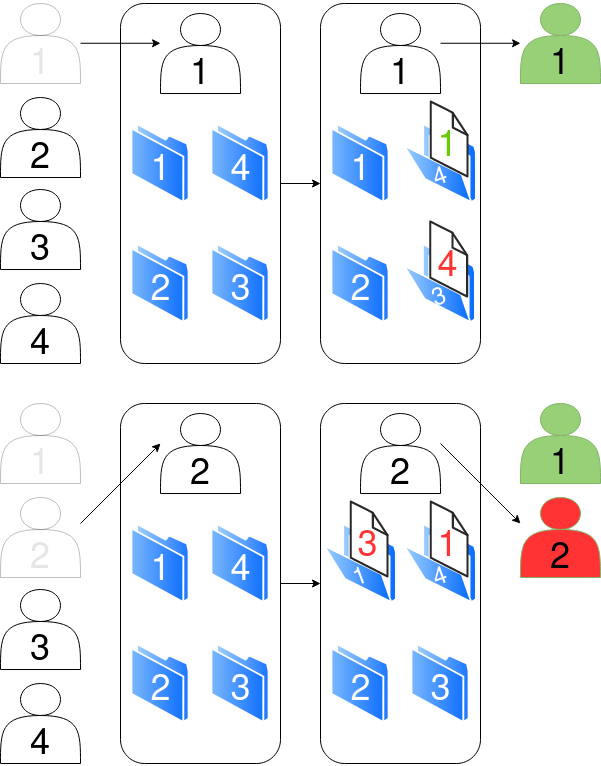
\includegraphics[height=0.3\textheight]{figures/indice_boites.png}
\caption{Le joueur 1 a trouvé la feuille correspondant à son numéro, il ne fera donc pas perdre l'équipe. Le joueur 2 n'a pas trouvé sa feuille, l'équipe sera donc annoncée perdante à la fin des passages.}
\end{figure}



\bibliographystyle{plainnat}  
\bibliography{sujets}

\end{document}